% 
\documentclass[cic,tc]{iiufrgs}

% Use unicode
\usepackage[utf8]{inputenc}   % pacote para acentuação

% Necessário para incluir figuras
\usepackage{graphicx}         % pacote para importar figuras

\usepackage{times}            % pacote para usar fonte Adobe Times
% \usepackage{palatino}
% \usepackage{mathptmx}       % p/ usar fonte Adobe Times nas fórmulas

\usepackage[alf,abnt-emphasize=bf]{abntex2cite}	% pacote para usar citações abnt

\usepackage{array}
% 
% Informações gerais
% 
\title{Implementação e Avaliação de um Mecanismo de Detecção de Ameaças em uma Ferramenta Smart Grid}

\author{Eitelvein}{Luiza dos Santos}

\advisor[Prof.~Dr.]{Schaeffer-Filho}{Alberto Egon}

% a data deve ser a da defesa; se nao especificada, são gerados
% mes e ano correntes
% \date{dezembro}{2015}

 \location{Porto Alegre}{RS}

% itens individuais da nominata podem ser redefinidos com os comandos
% abaixo:
% \renewcommand{\nominataReit}{Prof\textsuperscript{a}.~Wrana Maria Panizzi}
% \renewcommand{\nominataReitname}{Reitora}
% \renewcommand{\nominataPRE}{Prof.~Jos{\'e} Carlos Ferraz Hennemann}
% \renewcommand{\nominataPREname}{Pr{\'o}-Reitor de Ensino}
% \renewcommand{\nominataPRAPG}{Prof\textsuperscript{a}.~Joc{\'e}lia Grazia}
% \renewcommand{\nominataPRAPGname}{Pr{\'o}-Reitora Adjunta de P{\'o}s-Gradua{\c{c}}{\~a}o}
% \renewcommand{\nominataDir}{Prof.~Philippe Olivier Alexandre Navaux}
% \renewcommand{\nominataDirname}{Diretor do Instituto de Inform{\'a}tica}
% \renewcommand{\nominataCoord}{Prof.~Carlos Alberto Heuser}
% \renewcommand{\nominataCoordname}{Coordenador do PPGC}
% \renewcommand{\nominataBibchefe}{Beatriz Regina Bastos Haro}
% \renewcommand{\nominataBibchefename}{Bibliotec{\'a}ria-chefe do Instituto de Inform{\'a}tica}
% \renewcommand{\nominataChefeINA}{Prof.~Jos{\'e} Valdeni de Lima}
% \renewcommand{\nominataChefeINAname}{Chefe do \deptINA}
% \renewcommand{\nominataChefeINT}{Prof.~Leila Ribeiro}
% \renewcommand{\nominataChefeINTname}{Chefe do \deptINT}

% 
% palavras-chave
% iniciar todas com letras minúsculas, exceto no caso de abreviaturas
% 
\keyword{smart grid}


%\settowidth{\seclen}{1.10~}

% 
% inicio do documento
% 
\begin{document}

% folha de rosto
% às vezes é necessário redefinir algum comando logo antes de produzir
% a folha de rosto:
% \renewcommand{\coordname}{Coordenadora do Curso}
\maketitle

% dedicatoria
% \clearpage
% \begin{flushright}
%     \mbox{}\vfill
%     {\sffamily\itshape
%       ``If I have seen farther than others,\\
%       it is because I stood on the shoulders of giants.''\\}
%     --- \textsc{Sir~Isaac Newton}
% \end{flushright}

% agradecimentos
%\chapter*{Agradecimentos}
%Agradeço ao \LaTeX\ por não ter vírus de macro\ldots



% resumo na língua do documento
\begin{abstract}
    Resumo em português.
\end{abstract}

% resumo na outra língua
% como parametros devem ser passados o titulo e as palavras-chave
% na outra língua, separadas por vírgulas
\begin{englishabstract}{Implementation and Evaluation of a Threat Detection Mechanism in a Smart Grid Tool}{Smart Grid}
    Abstract in English.
\end{englishabstract}

% lista de figuras
% \listoffigures

% lista de tabelas
% \listoftables

% lista de abreviaturas e siglas
% o parametro deve ser a abreviatura mais longa
\begin{listofabbrv}{SCADA}
    \item[SCI]   Sistema de Controle Industrial
    \item[CLP]   Controlador Lógico Programável
    \item[TIC]   Tecnologia da Informação e Comunicação
    \item[HMI]   Interface Homem-Máquina
    \item[DEI]   Dispositivos Eletrônicos Inteligente
    \item[UTR]   Unidade Terminal Remota
    \item[SCADA] Supervisory Control and Data Acquisition
    \item[ENISA] European Network and Information Security Agency
    \item[NIST]  National Institute of Standards and Technology
    \item[OCC]   One-Class Classification
	\item[AM]    Aprendizado de Máquina
	\item[SDI]   Sistema de Detecção de Intrusão
	\item[OCSVM] One-Class Support Vector Machine
	\item[SVM]  Support Vector Machine

    
\end{listofabbrv}

% idem para a lista de símbolos
% \begin{listofsymbols}{$\alpha\beta\pi\omega$}
%     \item[$\sum{\frac{a}{b}}$] Somatório do produtório
%     \item[$\alpha\beta\pi\omega$] Fator de inconstância do resultado
% \end{listofsymbols}

% sumario
\tableofcontents

\chapter{Introdução}
\section{Motivação}
\section{Objetivos}
\section{Contribuição}
\section{Estrutura do Trabalho}
\chapter{Fundamentação Teórica}
Neste capítulo, será estabelecida a fundamentação teórica dos tópicos abordados neste trabalho, afim de fornecer o entendimento dos conceitos e tecnologias que serão utilizados e apresentar o estado da arte em que se encontram. A seção \ref{secsg} introduz os smart grids, seu propósito, sua arquitetura e as ameaças que os afetam. Na seção \ref{secmec}, são abordados os mecanismos de segurança utilizados em smart grids. Finalmente, a seção \ref{sectools} apresenta as ferramentas existentes para simulação de ambientes smart grid e sistemas SCADA.

\section{Smart Grids}
\label{secsg}
Smart Grids combinam redes de energia elétrica com estruturas de comunicação, baseadas em Tecnologia de Informação e Comunicação (TIC), que provêm um meio de troca de dados entre os componentes envolvidos no processo de produção, distribuição e consumo de energia. Como suas principais características, podem ser mencionados o fluxo bidirecional de energia elétrica entre produtores e consumidores e a incorporação de uma infraestrutura de comunicação, também bidirecional, que provê uma maior capacidade de automação à rede \cite{2013survey}. Através de recursos e técnicas como monitoramento em tempo real, automação e controle de dispositivos, autoavaliação e autorecuperação, integração com de fontes de energia alternativas e mecanismos de segurança física e cibernética, Smart Grids imbuem a rede elétrica com maior confiabilidade, eficiência e segurança \cite{li2012securing}.
No restante desta sessão, são apresentados: as motivações para o uso de smart grids, em \ref{subsecmotiv}, sua arquitetura, em \ref{subsecarq}, e as ameaças às quais são suscetíveis, em \ref{subsecthreats}.

\subsection{Motivação}
\label{subsecmotiv}

A  infraestrutura de comunicação dos Smart Grids incorpora uma grande diversidade de benefícios ao sistema de produção, distribuição e consumo de energia. Dados coletados pela IMA podem ser utilizados para melhorar a eficiência e o desempenho da distribuição de energia, identificando picos de consumo e pontos de desperdício na rede, além de fornecer aos usuários informações detalhadas sobre seu consumo de energia, levando-os a um consumo mais eficiente. Uma maior automação da rede de distribuição leva à diminuição dos custos operacionais, pois seu funcionamento torna-se mais independente da mão de obra envolvida, que, por sua vez, pode executar suas tarefas com mais eficiência. A capacidade de comunicação entre diversas entidades e o fluxo bidirecional de energia possibilitam uma utilização cada vez maior de recursos de energia distribuídos, incentivando o surgimento de fontes de geração de energia renovável, como solar e eólica. Entidades consumidoras podem também ser produtoras de energia, permitindo que microprodutores forneçam energia à rede simultaneamente a grandes produtores \cite{2013survey}.

A capacidade de autoavaliação e autoajuste em redes elétricas e outras infraestruturas críticas, como sistemas de transporte e financeiros, é de imensa importância. Devido à modernização das tecnologias utilizadas, essas infraestruturas têm seus sistemas cada vez mais interconectados, aumentando o risco de falhas em cascata de grandes proporções. A demanda crescente por uma distribuição de energia mais eficiente e confiável traz a necessidade de aperfeiçoar métodos e ferramentas que forneçam às redes elétricas a capacidade de se autoregular e sofrer o menor impacto possível na ocorrência de sobrecarga, mal funcionamento ou ataques maliciosos \cite{massoud2005toward}.

\subsection{Arquitetura}
\label{subsecarq}

A produção de energia em um smart grid está distribuída em diversas fontes, que incluem usinas fixas e móveis e microprodutores. A energia elétrica é transportada das usinas de geração até as subestações de transmissão através de cabos de alta tensão, e então é transmitida, assim como a energia de outras fontes diversas, até as subestações de distribuição através de linhas de tensão variada. A partir das subestações de distribuição, finalmente, a energia é distribuída para consumo \cite{harb2013communication}.

Cada consumidor de um smart grid, em conjunto com um medidor inteligente e disjuntores de controle forma uma rede residencial. Redes residenciais, Dispositivos Eletrônicos Inteligentes (DEIs) e Unidades Terminais Remotas (UTRs) são agrupados em redes de comunidades que, por sua vez, são conectadas a produtores de energia e outros elementos do smart grid em uma área geográfica por uma rede regional \cite{li2012securing}. Controle e monitoramento da rede em cada região são realizados por centros de controle regionais que implementam sistemas de Controle de Supervisão e Aquisição de Dados – \textit{Supervisory Control and Data Acquisition (SCADA)}. Sensores inteligentes instalados ao longo de toda a extensão da rede coletam, em tempo real, informações detalhadas sobre o consumo de energia e os transmitem para centrais de dados, formando uma Infraestrutura de Monitoramento Avançada (IMA) \cite{2013survey}. A Figura \ref{fig:sgarchitecture} ilustra a arquitetura genérica da infraestrutura de um smart grid.

\begin{figure}[h]
   \caption{Arquitetura de um smart grid}
   \begin{center}
       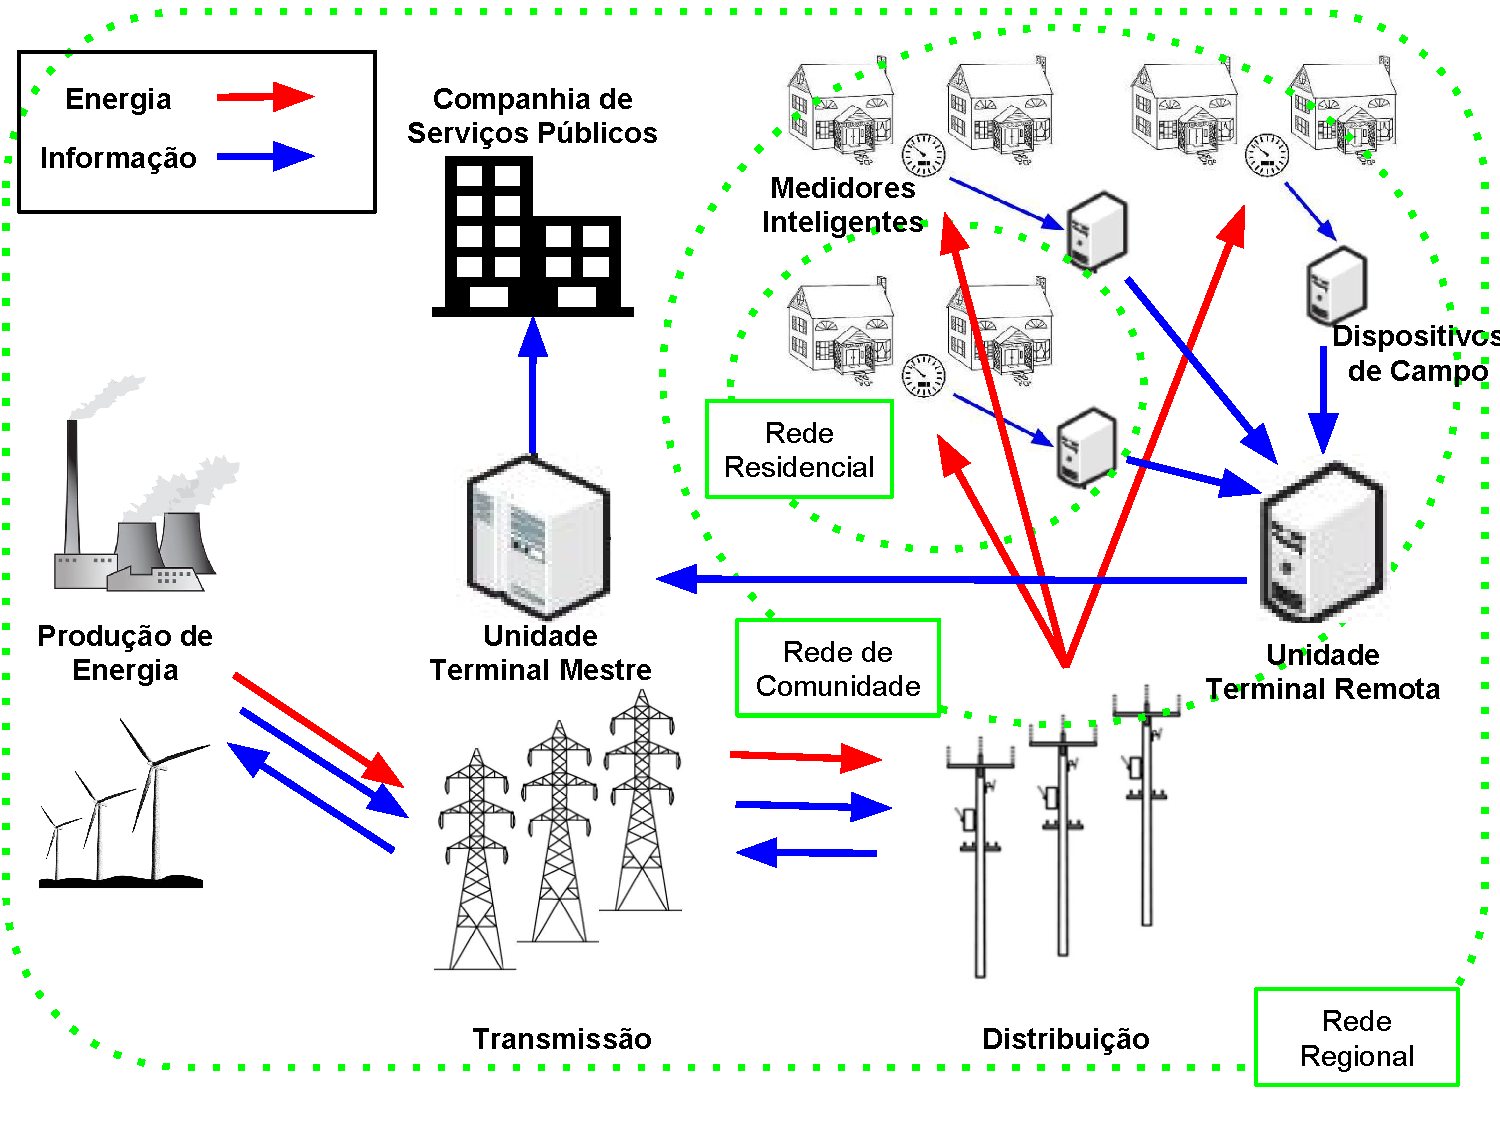
\includegraphics[width=26em]{smart_grid_arch}
   \end{center}
   \legend{Fonte: Autor}
   \label{fig:sgarchitecture}
\end{figure}


\subsection{Ameaças}
\label{subsecthreats}
A introdução de uma estrutura de comunicação autônoma e amplamente distribuída que ampara todo o funcionamento da rede elétrica expõe todo o sistema à possibilidade de ataques cibernéticos. A infraestrutura de comunicação, por ser desenvolvida sobre TIC, é inerentemente vulnerável a diversos tipos de ataque, que podem ser utilizados para manipular dados ou obstruir o funcionamento do sistema \cite{pin2012smart}. Medidores inteligentes também são potencialmente inseguros, estando vulneráveis a ataques de negação de serviço, roubo de informações de usuários e manipulação de dados \cite{ashford2011smartmeter}.

A evolução dos ataques cibernéticos e o risco que representam para infraestruturas críticas podem ser observados em fenômenos como o Stuxnet, um \textit{malware} desenvolvido para atacar controladores de sistemas industriais. O Stuxnet insere código ilegítimo na execução do controlador, que passa a ser executado em detrimento do código original, sem ser detectado, podendo levar à interrupção do serviço e danificar componentes do sistema atingido \cite{langner2011stuxnet}.

Uma taxonomia dos tipos de ataques cibernéticos em estruturas de comunicação de smart grids é apresentada em \cite{li2012securing}. Os autores descrevem quatro tipos de ataques, como apresentados na Tabela \ref{tbl:attacktypes}: ataques a dispositivos, ataques de dados, ataques de privacidade e ataques de disponibilidade de rede.

\subsubsection{Ataques a dispositivos}
Ataques a dispositivos têm como finalidade obter controle sobre um elemento do smart grid e utilizá-lo para um objetivo malicioso. De modo geral, servem a dois propósitos: fornecer os meios para um ataque de dados ou de disponibilidade ou, caso o dispositivo afetado possua funções de controle críticas, causar danos físicos ao sistema.

\subsubsection{Ataques de dados}
Ataques de dados configuram a tentativa de manipular os dados presentes na rede. Os dados manipulados podem ser informações de usuários ou sinais dos dispositivos de controle do smart grid. Seus usos variam de alterar dados de um usuário, para reduzir o valor da energia consumida, a eliminar sinais enviados por dispositivos de controle, para impedir o monitoramento e diagnóstico dos elementos da rede, o que pode levar à interrupção do funcionamento do sistema.

\subsubsection{Ataques de privacidade}
Ataques de privacidade têm o objetivo de obter informações privativas dos usuários. No caso dos smart grids, essas informações são os dados sobre o consumo de energia elétrica dos usuários, transmitidos pela rede de comunicação. Essas informações podem ser utilizadas para mapear dados privativos sobre a rotina dos usuários, que podem ser utilizados para fins maliciosos.

\subsubsection{Ataques de disponibilidade}
Ataques de disponibilidade de rede, ou ataques de negação de serviço, causam lentidão no tráfego de dados do smart grid através da sobrecarga da rede de comunicação e recursos computacionais. A velocidade da troca de dados é crítica para o funcionamento de um smart grid, e lentidão ou indisponibilidade do tráfego da rede podem causar prejuízos sérios aos seus usuários.

\begin{table}[h]
   \caption{Taxonomia dos tipos de ataques cibernéticos em smart grids}
   \centering
       \begin{tabular}{p{4cm}|p{8cm}}
         \hline
         Nome  &  Descrição\\
         \hline
         \hline
         Ataques a dispositivos & Têm como objetivo comprometer (controlar) um dispositivo da rede. Frequentemente, é o passo inicial de um ataque sofisticado.\\
         \hline
		Ataques de dados & Tentam inserir, alterar ou deletar dados no tráfego da rede para induzir o smart grid a tomar decisões erradas.\\
 \hline
		Ataques de privacidade & Têm como objetivo obter/inferir informações privadas do usuário analizando dados sobre a utilização de energia elétrica.\\
 \hline
		Ataques de disponibilidade de rede & Visam esgotar ou sobrecarregar os recursos de comunicação e computacionais do smart grid para causar atraso ou falha de comunicação. \\
         \hline
       \end{tabular}
   \legend{Fonte: \cite{li2012securing}}
\label{tbl:attacktypes}
\end{table}

\section{Mecanismos de Segurança}
\label{secmec}
Garantir confiabilidade e segurança é um grande desafio no desenvolvimento dos smart grids. O desacoplamento das funcionalidades de controle e comunicação dos dispositivos elétricos e a modularização dos subsistemas leva a uma inevitável perda de confiabilidade. Componentes passam a ser originários de diferentes fabricantes, introduzindo margem à incompatibilidades e falhas de comunicação. A agregação de fontes de energia distribuída, incluindo usinas de geração instáveis, levarão a fluxos de energia reversos e variações de voltagem. Ataques maliciosos podem ser direcionados tanto à rede elétrica física quanto à rede de comunicação \cite{li2012securing}. Apesar da existência de uma vasta gama de tecnologias de segurança voltadas à TIC, essas medidas de segurança não são capazes de resguardar o sistema contra ataques desenvolvidos para atingir sistemas SCADA, medidores inteligentes e outros componentes do smart grid \cite{carcano2011multidim}.
A seguir, são apresentados alguns mecanismos de segurança comumente utilizados em smart grids. Em \ref{subsecnormas}, são introduzidas as normas de segurança documentadas para smart grids, e \ref{subsecmecs} aborda mecanismos de detecção de intrusão.

\subsection{Normas de Segurança}
\label{subsecnormas}
A maior parte dos esforços para promover o desenvolvimento de smart grids mais seguros se concentra em normas e padrões de segurança. O conjunto de diretrizes de segurança NISTIR 7628 \cite{nistir7628}, desenvolvido pelo Instituto Nacional de Padrões e Tecnologia dos Estados Unidos - National Institute of Standards and Technology (NIST), apresenta um panorama geral de orientações, métodos e regulamentações para prover segurança cibernética a sistemas de controle industriais e automação. Entretanto, fatores como a complexidade do smart grid, sua ampla distribuição geográfica e sua larga escala fazem com que as práticas descritas pelas normas de segurança, como o uso de criptografia e autenticação nas interfaces de comunicação entre subsistemas, não sejam o bastante para garantir que o sistema estará seguro contra usuários maliciosos. Em \cite{chan2013cybersecurity}, os autores encontraram vulnerabilidades ao aplicarem o NISTIR 7628 a uma infraestrutura de carregamento de um veículo elétrico, demonstrando que os padrões de segurança descritos não são suficientes para garantir a segurança de um smart grid.

\subsection{Mecanismos de Detecção de Intrusão}
\label{subsecmecs}
Sistemas de Detecção de Intrusão (SDI) são aptos a detectar ataques lançados através de dispositivos internos do sistema que tenham sido comprometidos, reconhecendo o comportamento padrão de um sistema e identificando ataques a partir da premissa de que as ações de um atacante diferem do funcionamento convencional do sistema \cite{li2012securing}. Todavia, SDIs tradicionalmente desenvolvidos para TIC falham em suprir os requisitos de segurança de sistemas SCADA, e mecanismos voltados para satisfazer as necessidades desses sistemas ainda não estão suficientemente amadurecidos. Em \cite{coutinho2009anomaly}, os autores apresentam uma técnica de detecção de anomalias para centros de controle de infraestruturas críticas, utilizando o Algoritmo de Classificação de Conjuntos Irregulares, capaz de identificar dados corrompidos introduzidos em um sistema de energia elétrica de seis barramentos. Uma abordagem à detecção de intrusão em sistemas SCADA baseada em Análise de Estado Crítico e Proximidade de Estados é analisada em \cite{carcano2011multidim}. \cite{tsang2005multi} introduz um SDI multi agente, baseado no Modelo de Clusterização da Colônia de Formigas, para detecção descentralizada de anomalias em redes distribuídas.

\subsubsection{Classificação de Tráfego com algoritmos de Aprendizado de Máquina}
Algoritmos de Aprendizado de Máquina têm sido utilizados para a classificação de tráfego internet por por possuírem diversas características vantajosas para a tarefa. Enquanto técnicas de classificação de tráfego tradicionais dependem da inspeção do conteúdo de pacotes, mecanismos baseados em AM classificam os dados através de atributos que podem ser observados externamente, como tamanho dos pacotes e tempo entre a chegada de pacotes, criando padrões estatísticos. Há benefícios consideráveis nessa abordagem: o campo de dados do pacote deixa de ser obrigatoriamente visível  (os dados podem estar criptografados, por exemplo), e o classificador não precisa conhecer a sintaxe dos dados nos pacotes de cada aplicação \cite{nguyen2008survey}.

Primeiramente, a tarefa de classificação utilizando AM requer que atributos sejam definidos. Atributos são características dos fluxos de pacotes, como tamanho máximo e mínimo de pacote e tempo médio entre chegada de pacotes, que serão utilizados para selecionar instâncias de dados de tráfego. É necessário, então, treinar o algoritmo classificador, associando conjuntos de atributos com classes de tráfego definidas. Através da etapa de treinamento, o algoritmo gera o conjunto de regras que será utilizado para determinar a qual classe pertence uma determinada entrada. Finalmente, utilizando o conjunto de regras geradas no treinamento, o classificador pode receber dados de tráfego desconhecidos e identificar a que classe pertencem \cite{nguyen2008survey}.

\section{Ferramentas de Simulação}
\label{sectools}

A fim de realizar a implementação e a avaliação do SDI proposto neste trabalho, é necessário utilizar uma ferramenta que permita a simulação da estrutura de comunicação de um smart grid. São apresentadas, a seguir, algumas ferramentas que possibilitam a simulação de tráfego de dados entre componentes SCADA. Algumas ferramentas suportam apenas simulações do fluxo de dados em componentes específicos, como o CLP, enquanto outras permitem a simulação de estruturas mais completas, com tráfego de dados entre diversos componentes.

\subsection{VirtuaPlant}
VirtuaPlant \cite{virtuaplantwebsite} é um simulador de Sistemas de Controle Industriais (SCI). Possui uma interface gráfica chamada World View que simula o efeito das ações do sistema de controle sobre um recurso virtual utilizando protocolo Modbus. O recurso é representado por uma fábrica que enche garrafas.
	
O Controlador Lógico Programável (CLP) é implementado sobre a biblioteca pymodbus, que roda em uma thread separada no componente World View e compartilha seu contexto, que contém registradores, entradas e valores, com as funções do World View para simular recursos sendo conectados ao controlador. A Interface Homem-Máquina (HMI) utiliza GTK3 e executa o cliente pymodbus em uma thread separada, que conecta com o servidor através de TCP/IP, obtendo leituras constantes dos valores do servidor, isto é, do CLP.

A ferramenta VirtuaPlant fornece uma variedade de scripts de ataque ao CLP. Entretanto, não permite a definição de novos dispositivos, não sendo possível a definição de novas topologias. Também não possibilita a modelagem de elementos da infraestrutura de comunicação, já que a simulação engloba apenas a leitura e escrita dos valores do controlador PLC.

\subsection{mosaik}
O mosaik \cite{mosaikwebsite} permite usar diversos simuladores existentes em um contexto comum para realizar uma simulação coordenada de um cenário, que representa um conjunto de componentes de smart grid. Oferece uma API para os simuladores se comunicarem com ele e possui handlers para cada tipo de processo dos simuladores.
	
A ferramenta permite a modelagem de diferentes cenários envolvendo esses simuladores, possibilitando a criação de novos objetos e definição de novas topologias. A biblioteca SimPy é utilizada para a simulação coordenada de cenários, e a execução da simulação é feita executando passos em cada simulador ao longo do tempo. Cada simulador executa o seu próprio processo e laço de eventos, enquanto o Mosaik sincroniza esses processos e gerencia a troca de dados entre eles. Através da combinação com outros simuladores, é possível simular uma estrutura TIC.

O protocolo de comunicação entre o mosaik e os simuladores é definido por uma API. Existem duas versões da API: alto nível e baixo nível. A API baixo nível utiliza sockets TCP para estabelecer a comunicação entre o mosaik e os simuladores através da troca de mensagens JSON. A API alto nível, atualmente disponível nas linguagens Python e Java, fornece o encapsulamento dessa comunicação em uma classe abstrata, onde as mensagens trocadas entre os simuladores e o mosaik são implementadas como métodos.

A criação de cenários de simulação é feita por uma API que permite iniciar simuladores e instanciar modelos a partir deles, criando um conjunto de entidades. É possível conectar as entidades entre si para estabelecer a troca de dados entre elas.

O gerenciador de simuladores é responsável por iniciar e gerenciar os processos dos simuladores e a comunicação entre eles. Permite iniciar novos processos de simuladores, conectar a processos que já estão em execução e, no caso de simuladores desenvolvidos em Python, também permite importar módulos de simuladores e executá-los durante a execução do processo.

Em \cite{wermann2015astoria}, os autores apresentam o framework ASTORIA, desenvolvido a partir da integração do mosaik com um simulador de redes, que permite a especificação e execução de simulações customizadas de ambientes smart grids. Além disso, permite definir ataques, como Negação de Serviço, ao ambiente simulado e avaliar seu impacto na estrutura do smart grid.

\subsection{SCADASim}
A ferramenta SCADAsim \cite{scadasimart} é um framework para construção de simulações SCADA. Possui um conjunto de módulos que representam os componentes SCADA, como RTUs, PLCs e MTUs, e implementa os protocolos Modbus TCP e DNP3. Permite a integração de componentes externos e componentes internos simultaneamente através do conceito de Gates, que são objetos que conectam um ambiente externo com o ambiente da simulação.

É baseado em 3 componentes principais: SSScheduler, SSGate e SSProxy.  SSScheduler é um escalonador em tempo real que permite controlar e sincronizar mensagens recebidas. Gerencia uma lista de instâncias do componente SSGate, que são responsáveis por enviar e receber mensagens de um ambiente externo, garantindo a sincronização das mensagens entre dois ambientes. SSGate fornece conexão com o ambiente externo através de um protocolo, que é utilizado para se comunicar com os componentes SCADA externos. Atualmente os protocolos disponíveis são: ModbusGate, DNP3Gate e HTTPGate. SSProxy representa um dispositivo real ou aplicação externa que interage com os objetos simulados e com um SSGate, que direciona suas mensagens para componentes externos.

Os protocolos são gerenciados de dois modos. Os protocolos utilizados dentro do ambiente do simulador para comunicação entre componentes da simulação são chamados de protocolos simulados. Os protocolos utilizados para comunicação entre dispositivos e aplicações externas e os SSGates são chamados de protocolos originais. No ambiente interno da simulação, toda a comunicação entre os componentes utiliza versões simuladas dos protocolos SCADA. O framework possui uma biblioteca de protocolos SCADA originais e simulados, contendo: Modbus TCP, DNP3 TCP e HTTP.

O simulador SCADASim permite, através dos módulos integrados de componentes SCADA, criar componentes e definir topologias, além de possibilitar a integração com componentes reais através da API. Possui, também, uma biblioteca com alguns tipos de ataques comuns à estruturas SCADA, como worm e DDoS. Não suporta, todavia, a modelagem de elementos de geração de energia, presentes em um smart grid.

\subsection{Modbus PLC Simulator}
O Modbus PLC Simulator \cite{plcsimwebsite} é um simulador de CLP baseado na ferramenta Modbus Slaves. O Modbus Slaves é uma ferramenta que permite simular até 32 dispositivos simultaneamente. Os dados contidos nos dispositivos escravos (slaves) são acessíveis à aplicação mestre. Permite monitoramento de tráfego serial. Cada instância de escravo pode ser configurada para representar dados de um mesmo nodo ou de nodos diferentes.

A ferramenta suporta os protocolos Modbus TCP/IP, Modbus RTU (serial) e AB-DF1. Funciona criando uma thread de comunicação com interface para a API de comunicação e controla um bloco de RAM que funciona como a memória do CLP.

O Modbus PLC Simulator possibilita a simulação da troca de dados entre um dispositivo CLP, representado pela aplicação mestre, e outros dispositivos, não fornecendo suporte, entretanto, para os demais aspectos da comunicação TIC, como modelagem de topologias e de dispositivos da infraestrutura de rede.


\subsection{Comparação entre ferramentas de simulação}

O SDI proposto neste trabalho visa realizar a detecção de anomalias em uma rede SCADA através da classificação dos dados de tráfego em tempo real. Para que esta solução seja possível, o único requisito estritamente necessário à escolha da ferramenta a ser utilizada é que ela deve ser capaz de simular o tráfego de dados entre componentes de uma estrutura SCADA. Caso contrário, não será possível realizar a classificação do tráfego entre componentes. Dito isso, outras características são interessantes para realizar uma simulação mais completa, que gere cenários mais próximos a um smart grid real, como a modelagem de componentes e a definição de topologias. A Tabela \ref{tbl:ex1} apresenta uma comparação entre as ferramentas de simulação previamente abordadas utilizando os seguintes critérios:
\begin{itemize}
\item{Simulação da infraestrutura TIC}: A ferramenta permite a simulação de uma estrutura TIC. É um requisito obrigatório da ferramenta a ser escolhida, pois é necessário simular o tráfego de dados entre componentes SCADA.
​\item{Simulação de produção e consumo de energia}: A simulação de valores de produção e consumo de energia permite que o ambiente simulado seja mais próximo ao ambiente real de um smart grid.
\item{Elementos modeláveis}: Quais elementos da simulação podem ser modelados. Quanto maior a flexibilidade para modelar elementos, mais próxima à estrutura de um smart grid podemos tornar a simulação.
​\item{Protocolos de rede}: A utilização de um dos protocolos comumente utilizados em redes SCADA torna possível classificar os dados de tráfego de forma similar a um smart grid real.
​\item{Modelagem de troca de pacotes de rede e informações de energia}: Como é realizada a modelagem do tráfego e do fluxo de energia elétrica na simulação. Idealmente, a modelagem deve ter um grau abstração que torne o uso da ferramenta simples.
​\item{Definição de novas topologias} A possibilidade de definir novas topologias possibilida a simulação de cenários com configuração semelhante à de um smart grid.
​\item{Criação e simulação de ataques} Definir e executar ataques sobre a estrutura simulada é uma maneira eficiente de avaliar o SDI a ser implementado.
\end{itemize}


\begin{table}[h]
    \caption{Comparação entre ferramentas de simulação}
    % OBS: não use \begin{center}, pois este aumenta o espaçamento entre a caption/legend e a tabela
    % Para figuras, a aparência é melhor com o espaçamento extra
    \centering
    \scriptsize
    % \setstretch{0.8}
        \begin{tabular}{m{2.4cm}|m{2.4cm}|m{2.4cm}|m{2.4cm}|m{2.4cm}}
          \hline
           & \textit{VirtuaPlant} & \textit{mosaik} & \textit{SCADASim} & \textit{Modbus PLC Simulator} \\
          \hline
          \hline
          Simulação da infraestrutura TIC & N/D & API permite integração com simuladores de rede & Componente SSGate simula estrutura de comunicação & N/D \\
          \hline
          Simulação de produção e consumo de energia & N/D & Modelado pelo simulador PYPOWER & N/D & N/D \\
          \hline
          Elementos modeláveis & Leitura e escrita de valores do CLP & Infraestrutura SCADA, topologia da rede, consumo e geração de energia & Infraestrutura SCADA & Apenas tráfego de dados entre componentes e CLP \\
          \hline 
          Protocolos de rede & Modbus & API para integração com simuladores de rede & Modbus e DNP3 & Modbus \\
          \hline
          Modelagem de troca de pacotes de rede e informações de energia & N/D & 	Através dos simuladores de rede integrados & Modelagem realizada pelo componente SSGate & N/D \\
          \hline
          Definição de novas topologias & N/D & Permite definição de componentes e topologias & Permite definição de componentes e topologias & N/D \\
          \hline
          Criação e simulação de ataques & Inclui ataques que atingem os dados do CLP & Framework ASTORIA inclui definição e simulação de ataques à estrutura SCADA & Inclui biblioteca de ataques a componentes da estrutura SCADA & Possível desenvolver ataques para o componente CLP \\
          \hline
        \end{tabular}
    \legend{Fonte: O Autor}
    \label{tbl:ex1}
\end{table}

A partir da comparação entre as ferramentas, é possível analisar qual é mais adequada para o propósito deste trabalho. Apesar de permitirem a leitura e escrita de dados em componentes SCADA, os simuladores VirtuaPlant e Modbus PLC Simulator não possibilitam a simulação da infraestrutura TIC presente em um smart grid. Ambos os simuladores mosaik e SCADASim permitem a simulação da infraestrutura TIC do sistema SCADA, a definição de novas topologias e a modelagem de seus componentes de forma suficientemente simples. O mosaik, no entanto, permite a simulação da rede de energia elétrica presente em um smart grid, enquanto o SCADASim simula apenas a rede de comunicação.
Apesar de a simulação de um ambiente smart grid através do mosaik requisitar a integração com um simulador de redes, o framework ASTORIA implementa essa integração e permite a simulação tanto da rede elétrica quanto da rede de comunicação presentes em um smart grid, além de fornecer ataques que podem ser executados sobre a simulação. Deste modo, o framework ASTORIA foi escolhido como ferramenta para simulação do ambiente smart grid neste trabalho.

\chapter{Modelagem e Desenvolvimento}
O problema proposto por este trabalho consiste em implementar um mecanismo de detecção de intrusão e avaliá-lo utilizando uma ferramenta que simule a infraestrutura de um smart grid. Para isso, é necessário desenvolver um SDI e integrá-lo à ferramenta de simulação, de modo que o SDI possa receber, em tempo real, dados do ambiente smart grid e operar sobre eles.
 
Neste capítulo, serão apresentadas a modelagem e as ferramentas utilizadas para o desenvolvimento de uma solução para problema proposto. A Seção \ref{secastoria} contém mais informações sobre o framework ASTORIA, utilizado para configurar as simulações do ambiente smart grid. A Seção \ref{secsdi} descreve a modelagem do SDI proposto e as tecnologias utilizá-das para desenvolvê-lo.
 
\section{Simulação da estrutura de smart grid com Framework ASTORIA}
\label{secastoria}
 
O Framework ASTORIA, descrito pelos autores em \cite{wermann2015astoria}, permite modelar simulações de ambientes smart grid, definir e executar ataques nesses ambientes e avaliar seus resultados e o comportamento do sistema.
O propósito da utilização do mosaik é agregar diversos simuladores em um contexto comum, para que sua execução sincronizada possa criar um ambiente de smart grid. Para isso, é necessário conectar as ferramentas que farão a simulação dos componentes dos smart grid.
 
A simulação da rede elétrica é realizada pelo PYPOWER, uma ferramenta nativamente integrada ao mosaik. Para realizar a simulação do componente de comunicação do smart grid, foi realizada a integração do mosaik com o simulador de redes ns-3.
O restante desta seção descreve o framework ASTORIA, seu funcionamento e as simulações produzidas por ele. Em \ref{subsecns3}, é abordado o simulador de redes ns-3, utilizado para compor os elementos de comunicação da simulação. \ref{subsecinteg} fala sobre a integração entre as ferramentas que compõe o framework, os simuladores mosaik, ns-3 e PYPOWER. Por fim, \ref{subsecestrut} mostra a estrutura das simulações produzidas pelo framework.
 
\subsection{ns-3}
\label{subsecns3}
 
O ns-3 \cite{nsnam} é um simulador de redes que funciona mantendo uma lista de eventos que devem ser executados, sequencialmente, em determinados tempos da simulação.  Desenvolvido para fins de estudo e pesquisa, está disponível publicamente para uso, e sua estrutura suporta simulações tanto de redes baseadas em IP quanto de redes não baseadas em IP. Também permite a interação entre simulações e dispositivos reais, possibilitando o envio de pacotes gerados pelo simulador para dispositivos de uma rede real.
 
O ns-3 utiliza possui diversas classes que representam abstrações dos objetos reais de uma rede.
 
\begin{itemize}
\item{Nó}: Um nó, modelado pela classe Node, representa um dispositivo computacional, também referido como host ou terminal em um rede Internet.
\item{Aplicação}: Uma aplicação é um programa de usuário que gera alguma atividade a ser simulada. Como o simulador não possui conceito de programas de sistema, existem apenas as aplicações que são executadas nos nós, representados pela classe Application.
\item{Canal de Comunicação}: Canais de comunicação são objetos que conectam sub-redes e os nós, formando o meio de comunicação entre os elementos. São descritos pela classe Channel.
\item{Dispositivo de Rede}: Um dispositivo de rede é acoplados a um nó para permitir que ele se comunique com outros nós através dos canais de comunicação. É modelado pela classe NetDevice e simula tanto os elementos de hardware quanto os de software de um dispositivo de rede real. É possível conectar um nó a diversos canais utilizando múltiplos dispositivos de rede.
\item{Assistentes de Topologia}: Assistentes de Topologia são objetos que combinam diversas operações distintas que são necessárias para a execução da simulação, como a criação e interconexão de objetos, com o objetivo de oferecer um modelo simplificado para a simulação.
\end{itemize}
 
\subsection{Integração entre as ferramentas}
\label{subsecinteg}
 
A simulação de um smart grid utilizando o ASTORIA acontece através da integração das funcionalidades de três ferramentas: PYPOWER, que realiza a simulação da rede de energia elétrica, ns-3, que simula a rede de comunicação da estrutura SCADA, e mosaik, que sincroniza a execução das demais ferramentas.
 
O PYPOWER \cite{pypower},  é uma ferramenta que implementa as funcionalidades do MATPOWER \cite{matpower} na linguagem Python e permite simular cenários de fluxo de energia elétrica, fornecendo os dados de produtores e consumidores de energia. O PYPOWER permite a simulação de uma estrutura de rede elétrica e gera dados de produção e consumo em tempo real. Esses dados são fornecidos, através do mosaik, para a rede de comunicação. Como o PYPOWER já é originalmente integrado ao mosaik, os dois já estão conectados e não há necessidade de implementar a troca de dados entre eles.
 
A integração do mosaik com o simulador ns-3, utilizado para compor o elemento de comunicação da simulação do smart grid, foi feita através da mosaik Sim API, que possibilita a sincronização com outros simuladores. A comunicação entre as ferramentas é realizada através de sockets TCP e mensagens JSON. As mensagens seguem o padrão requisição-resposta e são compostas por um cabeçalho, que carrega o número de bytes no corpo, e pelo corpo da mensagem, que contém o tipo, o identificador e o conteúdo da mensagem. As mensagens a seguir são utilizadas pelo mosaik para comunicação com os simuladores.
 
Chamadas enviadas pelo mosaik para os simuladores:
 
\begin{itemize}
\item \emph{init()}: Inicialmente, quando a conexão é estabelecida, o mosaik chama o método \emph{init()}, que passa parâmetros globais ao simulador, que responde com informações sobre ele.
\item \emph{create()}: As simulaçoes podem ser instanciadas pelo mosaik utilizando o método \emph{create()}, que também retorna dados sobre os objetos criados.
\item \emph{setup_done()}: A fase de configuração é encerrada pela chamada do método \emph{setup_done()}, que é seguido por múltiplas chamadas do método step().
\item \emph{step()}: Cada chamada de \emph{step()} feita pelo mosaik permite que o simulador avance uma etapa de simulação no tempo e execute eventos agendados para aquele instante. A chamada é retornada com o próximo instante de tempo em que o simulador deve performar a próxima ação.
\item \emph{get_data()}: Mensagens \emph{get_data()} podem ser enviadas para requisitar dados sobre alguma instancia.
\item \emph{stop()}: O envio da mensagem \emph{stop()} pelo mosaik para cada simulador indica que ele deve ser encerrado.
\end{itemize}

As seguintes requisições assíncronas podem ser enviadas pelos simuladores, durante uma etapa da simulação, para o mosaik:

\begin{itemize}
\item \emph{get_data()}:​ ​​A mensagem \emph{get_data()} pode ser enviada​ por um simulador​ para obter dados de outras​ entidades​ ​presentes na simulação.
​\item \emph{set_data()}:​ Através da mensagem \emph{set_data()}, ​o simulador é capaz de​ ​modificar dados de outras entidades.
\item \emph{get_progress()}:​ ​​​A​ requisiçã​o​​​ \emph{get_progress()} é enviada​ ao mosaik​ para ​obter informações sobre o progresso da simulação.
​​\item \emph{get_related_entities()}:​ A requisição \emph{get_related_entities()} é utilizada pelos simuladores para obter informações sobre a topologia da simulação.
\end{itemize}

O ns-3 inicia a conexão com o mosaik através de um socket TCP e, por meio dessa conexão, é realizado o envio das mensagens, através das quais o mosaik sincroniza a execução dos dois simuladores, PYPOWER e ns-3, e fornece os dados da rede elétrica para a rede de comunicação.
 
A execução do mosaik é baseada em passos. Após a fase de configuração, em que é feita a inicialização dos simuladores e a criação das instâncias de simulação, é enviada para o ns-3 uma mensagem a cada passo de execução, contendo os dados referentes à produção e ao consumo de energia, gerados pelo PYPOWER. Ao receber a mensagem contendo esses dados, o ns-3 executa a etapa atual da simulação, responde a mensagem com o instante em que a próxima etapa de simulação deve ser executada e entra em espera até receber a próxima mensagem.

\subsection{Simulação do ambiente smart grid}
\label{subsecestrut}

A rede de energia elétrica é composta por nodos de geração, consumo e distribuição de energia. Os dados medidos nos componentes são gerados a partir de perfis de produção e consumo de energia presentes no simulador. A estrutura SCADA formada pela rede de comunicação é composta por sensores, RTUs e MTUs. Cada nodo de produção, distribuição e consumo presente na rede elétrica possui um nodo correspondente na rede de comunicação SCADA. Cada nodo de produção ou consumo está pareado com um sensor SCADA, enquanto os nodos de distribuição de energia estão pareados com as RTUs. As MTUs não possuem nenhum componente respectivo na rede elétrica, por serem um componente exclusivo da estrutura SCADA.
A Figura \ref{figsimulation} mostra a estrutura dos componentes na simulação do ambiente smart grid com o framework ASTORIA. Os dados recebidos por cada sensor SCADA contém informações sobre a produção e o consumo de energia da unidade associada a ele. As RTUs recebem os dados de todos os sensores conectados a elas, e então enviam todas as informações recolhidas para a MTU. A comunicação entre os componentes SCADA acontece através do protocolo modbus.

(inserir aqui imagem da estrutura dos componentes da simulação)
 
\section{Mecanismo de Detecção de Intrusão}
\chapter{Implementação e Análise de Resultados}
\section{Implementação do Sistema de Detecção de Intrusão}
\section{Execução dos Experimentos}
\section{Análise dos Resultados}
\chapter{Conclusão e Trabalhos Futuros}
\section{Resumo de Contribuições}
\section{Trabalhos Futuros}

% referências
% aqui será usado o environment padrao `thebibliography'; porém, sugere-se
% seriamente o uso de BibTeX e do estilo abnt.bst (veja na página do
% UTUG)
% 
% observe também o estilo meio estranho de alguns labels; isso é
% devido ao uso do pacote `natbib', que permite fazer citações de
% autores, ano, e diversas combinações desses

\bibliographystyle{abntex2-alf}
\bibliography{biblio}

\end{document}
